\section{Compile: supersession, not memory or structure}
\label{sec:compile}

\subsection{Setup}

We use HoH \citep{ouyang2025hoh}, a benchmark built from Wikipedia dynamic-fact edits mined via token-level diffs, so that every item ships both a current and a superseded passage. We pool all evidence from $n{=}300$ HoH queries into a single shared $628$-document corpus ingested in one fixed order, rather than giving each query its own mini-corpus, so that every system under test sees the same evolving-corpus ingestion problem. Seven arms are compared under a fixed Qwen2.5-14B reader: closed-book (no retrieval), full-context dump, vector RAG (dense retrieval, top-$k$), LightRAG \citep{guo2025lightrag} (a real graph-RAG system, unmodified), RAPTOR \citep{sarthi2024raptor} (a real tree-RAG system, unmodified), an LLM-Wiki compile (Karpathy-style: an LLM reads new documents and rewrites affected pages, resolving contradictions with newer-supersedes-older), and a label-free recency resolver (a lighter-weight baseline that reorders retrieved evidence by inferred recency without a full compile step). The metric is staleness error rate (SER): the fraction of queries answered using the superseded fact instead of the current one.

\subsection{Compiling with resolution beats retrieval, structure alone does not}

\begin{table}[t]
\centering
\small
\caption{Staleness error rate (SER, lower is better) by arm, HoH $n{=}300$, Qwen2.5-14B. LLM-Wiki resolves supersession at compile time; LightRAG and RAPTOR are real structured (graph/tree) RAG systems that accumulate rather than resolve.}
\label{tab:compile-arms}
\begin{tabular}{lccc}
\toprule
Arm & Mechanism & SER & Accuracy \\
\midrule
Closed-book & no retrieval & 0.043 & 0.06 \\
Full-context dump & no selection & 0.143 & -- \\
Vector RAG & flat, accumulate & 0.277 & -- \\
LightRAG \citep{guo2025lightrag} & graph, accumulate & 0.280 & -- \\
RAPTOR \citep{sarthi2024raptor} & tree, accumulate & 0.177 & -- \\
Label-free resolver & flat, resolve & 0.050 & 0.673 \\
LLM-Wiki (ours) & flat, resolve (compiled) & \textbf{0.007} & 0.910 \\
\bottomrule
\end{tabular}
\end{table}

Closed-book abstains rather than answering correctly (accuracy $0.06$), so its low SER reflects not-answering, not currency --- it is not a real competitor. Among arms that actually answer, LLM-Wiki's SER of $0.007$ is $25$--$40\times$ lower than vector RAG ($0.277$) and the two real structured systems, LightRAG ($0.280$) and RAPTOR ($0.177$).

The obvious confound is that LLM-Wiki has both more structure (a compiled, curated store) and a different update rule (resolve instead of accumulate) than vector RAG, so the improvement could be credited to either. We break this apart with a controlled $2\times2$ over structure (flat vs.\ graph) and update policy (accumulate vs.\ resolve): flat-accumulate SER $0.277$, flat-resolve $0.050$, graph-accumulate $0.137$, graph-resolve $0.003$. Holding structure fixed and switching only the update policy from accumulate to resolve cuts SER by $5$--$45\times$ in both the flat and graph conditions; holding the update policy fixed and adding graph structure does not reliably help (flat-resolve $0.050$ vs.\ graph-resolve $0.003$ is a further improvement, but flat-accumulate $0.277$ vs.\ graph-accumulate $0.137$ shows structure alone, without resolution, still leaves the majority of staleness error in place). The operative variable is \emph{recency-aware supersession resolution}, not memory, not graph structure, and not the presence of a compile step per se — a label-free resolver with no compile at all already gets most of the way there (SER $0.050$).

\paragraph{A currency certificate, not just a point estimate.} A single SER number invites overclaiming from a lucky sample. We additionally report a Clopper-Pearson $95\%$ one-sided upper confidence bound $\hat\varepsilon$ on SER for each arm (\Cref{fig:compile-cert}): resolving arms certify $\hat\varepsilon \le 0.08$ (LLM-Wiki $0.021$; label-free resolver $0.076$--$0.080$ after judge-noise correction), while every cumulative-index (accumulating) arm certifies only $\hat\varepsilon \ge 0.18$ even though its point estimate can look better on a given sample. This certificate --- and what it costs to tighten as a function of audit size $n$ --- becomes the building block for \S\ref{sec:certify}.

\begin{figure}[t]
\centering
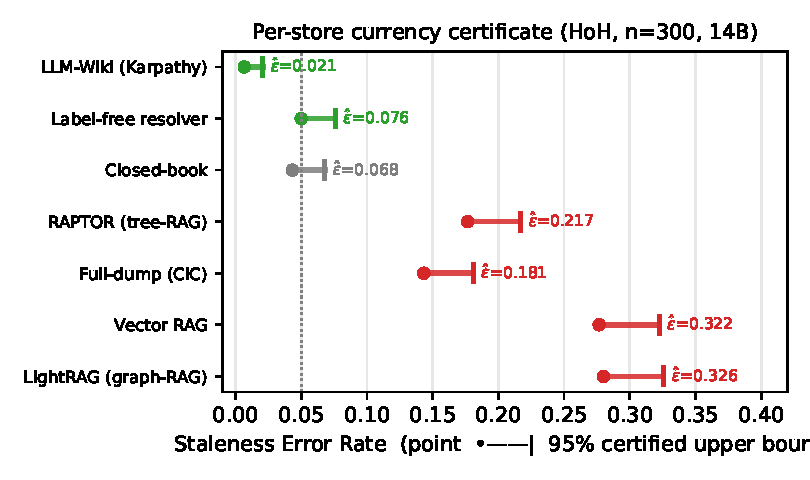
\includegraphics[width=0.48\linewidth]{figures/compile_certificate.pdf}
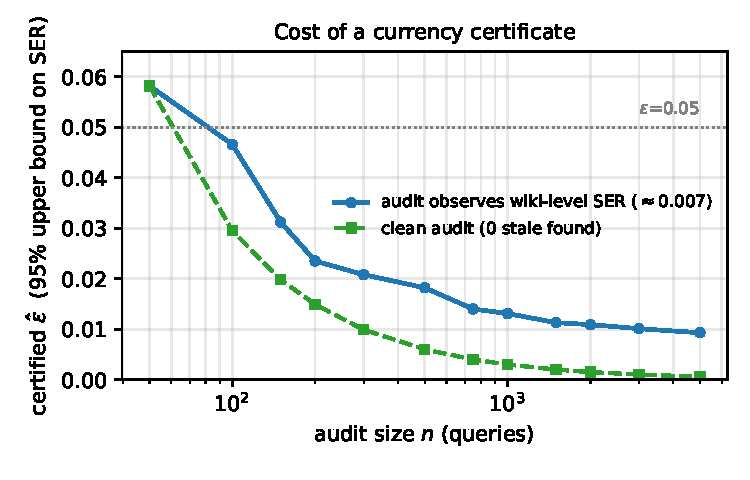
\includegraphics[width=0.48\linewidth]{figures/compile_samplesize.pdf}
\caption{Left: per-store currency certificate (point SER vs.\ $95\%$ Clopper-Pearson upper bound), resolving arms (green) vs.\ accumulating arms (red). Right: cost of tightening a currency certificate as audit size $n$ grows.}
\label{fig:compile-cert}
\end{figure}

\subsection{External validation: a different dataset, a different tool}
\label{sec:compile-external}

The result above uses one dataset (HoH), one reader model family, and our own compile harness. As an independent robustness check, we ran a second experiment on a different dataset (SciFact-Open \citep{scifact}, real PubMed abstracts, $75$ tracked SUPPORT claims plus $1500$ filler documents) using a driver that faithfully reproduces a real, independently-published third-party LLM-Wiki tool's update policy (a Hermes-style LLM-Wiki skill's documented rewrite instructions), rather than our own compile prompt. This tests whether ``iterated rewriting loses information'' is an artifact of our specific harness or a more general property of the compile-and-rewrite pattern.

\begin{table}[h]
\centering
\small
\caption{External validation on SciFact-Open, seed $=0$, single run per arm. $r_0{\to}r_T$ is retention at round $0$ vs.\ round $12$; rebuild is a fresh recompile at round $T$ with no rewrite history (the ceiling). Because arms were run independently, $r_0$ is not matched across arms --- relative retention $r_T/r_0$ is the fair cross-arm comparison.}
\label{tab:compile-external}
\begin{tabular}{lcccc}
\toprule
Arm & $r_0$ & $r_T$ & rebuild ceiling & $r_T/r_0$ \\
\midrule
Plain (large model) & 17.3\% & 13.3\% & 26.7\% & 77\% \\
Harness (rollback-wrapped, large) & 32.0\% & 29.3\% & 53.3\% & 92\% \\
Plain (small model) & 22.7\% & 2.7\% & 49.3\% & 12\% \\
\bottomrule
\end{tabular}
\end{table}

Three findings replicate qualitatively on a dataset and tool neither used for the HoH result. First, rewriting loses information even under a real, unmodified third-party update policy, on real scientific abstracts rather than one-fact wiki snippets. Second, the effect is model-size dependent and can be severe: the small model collapses to $12\%$ relative retention, essentially total loss, while the large model degrades but survives. Third, a cheap check-and-rollback wrapper (\S\ref{sec:maintain}'s LossGate logic applied externally, without retraining) slows relative decay substantially (92\% vs.\ 77\%) without eliminating it --- the same qualitative story as the certified maintenance result in \S\ref{sec:maintain}, obtained independently.

We report this honestly as a single-seed, same-model-self-judged (temperature $0$, no independent calibrated judge) robustness check, not a second headline result: the magnitude is dataset- and model-dependent, and even the rebuild ceiling here ($26.7$--$53.3\%$) is well below $100\%$, indicating this particular tool's extraction/synthesis pipeline is itself imperfect independent of rewriting. What it does establish is that the phenomenon is not specific to our benchmark, our prompt, or our judge.
